\chapter{整数論 - Number theory}

\index{number theory}

\key{整数論(Number theory)}は整数を研究する数学の分野です。
整数論は一見単純そうに見えるかもしれませんが、
整数に関わる多くの問題は非常に難しく、ですが興味深い分野です。

例として、次のような式を考えてみましょう。
\[x^3 + y^3 + z^3 = 33\]

実数の範囲では$x$, $y$,$z$の例を見つけるのは簡単で、例えば以下のものが思い浮かびます。
\[
\begin{array}{lcl}
x = 3, \\
y = \sqrt[3]{3}, \\
z = \sqrt[3]{3}.\\
\end{array}
\]
ところが、
\emph{整数(integers)}である $x$, $y$ and $z$を見つけるというのは未解決問題です。\cite{bec07}

この章では、整数論の基本的な概念とアルゴリズムに焦点を当てていきます。
この章では特に断らない限り、すべての数は整数であると仮定します。

\section{素数と因数 - Primes and factors}

\index{divisibility}
\index{factor}
\index{divisor}


$a$が$b$の因数であるとき、 $a \mid b$と表記し、そうでなければ$a \nmid b$と記載します。

例えば24の因数は1, 2, 3, 4, 6, 8, 12, 24です。

\index{素数 - prime}
\index{prime decomposition}

$n>1$である数が1または$n$以外の因数を持たない場合\key{素数}と呼びます。
例えば、7、19、41は素数ですが、35は$5 \cdot 7 = 35$なので素数ではありません。
$n>1$である数には、\key{素因数分解 - prime factorization}が唯一に存在します。
\[ n = p_1^{\alpha_1} p_2^{\alpha_2} \cdots p_k^{\alpha_k},\]
ここで、$p_1,p_2,\ldots,p_k$は異なる素数であり、$\alpha_1,\alpha_2,\ldots,\alpha_k$は正の数です。
84の素因数分解は次のようになります。
\[84 = 2^2 \cdot 3^1 \cdot 7^1.\]

ある数$n$の因数の個数を
\[\tau(n)=\prod_{i=1}^k (\alpha_i+1),\]
とします。
なぜなら、各素数$p_i$が
因数に何回現れるかを選ぶ方法は$\alpha_i+1$通りあるからです
。例えば、84の因子の数は、$\tau(84)=3 \cdot 2 \cdot 2 = 12$です。
実際に因数分解する と、1、2、3、4、6、7、12、14、21、28、42、84となります。

$n$ の \key{因数の和 - sum of factors} は
\[\sigma(n)=\prod_{i=1}^k (1+p_i+\ldots+p_i^{\alpha_i}) = \prod_{i=1}^k \frac{p_i^{a_i+1}-1}{p_i-1},\]
ここで、後者の式は幾何級数式(TODO: geometric progression formula)によります。
例えば、84の因数の和は次の通りとなります。
\[\sigma(84)=\frac{2^3-1}{2-1} \cdot \frac{3^2-1}{3-1} \cdot \frac{7^2-1}{7-1} = 7 \cdot 4 \cdot 8 = 224.\]

$n$の \key{因数の積 - product of factors} は
\[\mu(n)=n^{\tau(n)/2},\]
となります。
TODO:  because we can form $\tau(n)/2$ pairs from the factors,
each with product $n$.
84の因数の積は次のようなペアで示されます。
$1 \cdot 84$, $2 \cdot 42$, $3 \cdot 28$などなど。
この結果、因数は積は$\mu(84)=84^6=351298031616$となります。

\index{完全数 - perfect number}
$n=\sigma(n)-n$の場合、$n$は\key{完全数(perfect number)}と呼ばれます。
これは$n$が$1$から$n - 1$までの因数の和に等しい場合です。例えば、28は、$28=1+2+4+7+14$なので、完全数です。

\subsubsection{素数は無限に存在する - Number of primes}

素数が無限にあることを示します。
もし、素数の数が有限であれば、素数全ての集合である
$P=\{p_1,p_2,\ldots,p_n\}$を作ることができ、これはすべての素数を含みます。
例えば、$p_1=2$, $p_2=3$, $p_3=5$です。
ところが$P$全ての要素を使って以下のPに含まれるのよりも大きな素数を作ることができます。
\[p_1 p_2 \cdots p_n+1\]
これは矛盾するため、素数の数は無限となります。

\subsubsection{素数の密度 - Density of primes}

素数の密度とは、数字の中にどれくらいの頻度で素数が含まれているかのことです。
$\pi(n)$を1から$N$までに含まれる素数の数とします。
例えば、$\pi(10)=4$です。1から10までの間に$2、3、5、7$の4つの素数があることを意味します。

これは次のように近似的に示すことができます。
\[\pi(n) \approx \frac{n}{\ln n},\]
この式からわかる通り素数の密度は高いです。
例えば$1$ から $10^6$ の実際の素数の数は$\pi(10^6)=78498$であり、
$10^6 / \ln 10^6 \approx 72382$でおおよそ一致します。

\subsubsection{予想 - Conjectures}

素数に関する \emph{予想(conjectures)} がいくつも存在します。
これらのほとんどが正しいとされていますが証明はされていません。
例えば以下のような予想が有名です。

\begin{itemize}
\index{Goldbach's conjecture}
\item \key{ゴールドバッハ予想 - Goldbach's conjecture}:
$n > 2$は偶数である場合、$a$および$b$がともに素数であるような$n = a + b$の和で表すことができる。
\index{twin prime}
\item \key{双子の予想(TODO) (Twin prime conjecture)}:
$\{p,p+2\}$であるようなペアは無限に存在する。ただし、$p$と$p+2$は素数である。
\index{Legendre's conjecture}
\item \key{ルジャンドル予想 TODO (Legendre's conjecture)}:
$n^2$と$(n+1)^2$の間には必ず素数が存在する。ただし、$n$は正の整数である.
\end{itemize}

\subsubsection{基本的なアルゴリズム - Basic algorithms}

素数でない$n$は$a \cdot b$という積で表すことができるので$a \le \sqrt n$か$b \le \sqrt n$となり、
$2$ 以上 $\lfloor \sqrt n \rfloor$以下の因数を持ちます。
この性質を利用すれば、ある数が素数であるかどうかの判定および
ある数の素因数分解を$O(\sqrt n)$時間で求められます。

次の関数 \texttt{prime} は、
与えられた数$n$が素数かどうかを判定します。
この関数は$n$を$2$から$\lfloor \sqrt n \rfloor$の数で割ろうとし、
どれでも割り切れなければ$n$は素数だとします。

\begin{lstlisting}
bool prime(int n) {
    if (n < 2) return false;
    for (int x = 2; x*x <= n; x++) {
        if (n%x == 0) return false;
    }
    return true;
}
\end{lstlisting}

\noindent
次に示す関数\texttt{factors}は$n$の素因数分解を行います。
これは数を順に割れるか判定していき、割れた数をvectorに追加していきます。
この関数は$n$が$2$ から $\lfloor \sqrt n \rfloor$の因数を持たないようにします。
この処理が終わったのちに$n>1$であるならば、それは最後の素因数です。
\begin{lstlisting}
vector<int> factors(int n) {
    vector<int> f;
    for (int x = 2; x*x <= n; x++) {
        while (n%x == 0) {
            f.push_back(x);
            n /= x;
        }
    }
    if (n > 1) f.push_back(n);
    return f;
}
\end{lstlisting}

この関数は、その素因数で数を割った回数だけvectorに現れるます。
例えば、$24$について$24=2^3 \cdot 3$なので、
これを素因数分解した結果は$[2,2,2,3]$となります。

\subsubsection{エラトステネスの篩 - Sieve of Eratosthenes}

\index{sieve of Eratosthenes}

\key{エラトステネスの篩(ふるい)(sieve of Eratosthenes)}
%\footnote{Eratosthenes (c. 276 BC -- c. 194 BC) was a Greek mathematician.}
とは$2 \ldots n$の間の数が素数かどうかチェックし、
素数でない場合はその数の素因数を見つけることができる配列を構築する効率的な前処理アルゴリズムです。

このアルゴリズムは、インデックス$2,3,\ldots,n$を持つ配列の$\texttt{篩}$を構築します。
$\texttt{sieve}[k]=0$であるとき$k$が素であることを意味し、
$\texttt{sieve}[k] \neq 0$であるときは$k$が素でなく、
素因数の1つが$\texttt{sieve}[k]$であることを意味します。

このアルゴリズムは$2 \ldots n$を順番にを1回ずつみていきます。
新しい素数$x$が見つかると、
$x$の倍数($2x,3x,4x,\ldots$) は $x$で割れてしまうため素数ではないとマークします。

例えば$n=20$の場合は次のような配列がつくられます。

\begin{center}
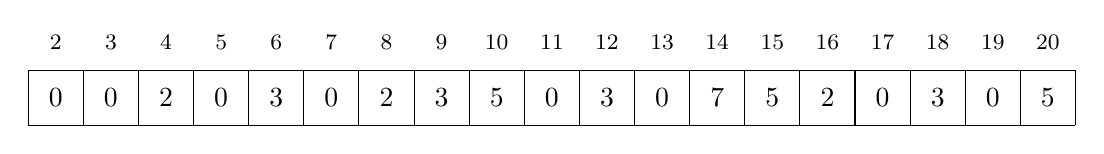
\begin{tikzpicture}[scale=0.7]
\draw (0,0) grid (19,1);

\node at (0.5,0.5) {$0$};
\node at (1.5,0.5) {$0$};
\node at (2.5,0.5) {$2$};
\node at (3.5,0.5) {$0$};
\node at (4.5,0.5) {$3$};
\node at (5.5,0.5) {$0$};
\node at (6.5,0.5) {$2$};
\node at (7.5,0.5) {$3$};
\node at (8.5,0.5) {$5$};
\node at (9.5,0.5) {$0$};
\node at (10.5,0.5) {$3$};
\node at (11.5,0.5) {$0$};
\node at (12.5,0.5) {$7$};
\node at (13.5,0.5) {$5$};
\node at (14.5,0.5) {$2$};
\node at (15.5,0.5) {$0$};
\node at (16.5,0.5) {$3$};
\node at (17.5,0.5) {$0$};
\node at (18.5,0.5) {$5$};

\footnotesize

\node at (0.5,1.5) {$2$};
\node at (1.5,1.5) {$3$};
\node at (2.5,1.5) {$4$};
\node at (3.5,1.5) {$5$};
\node at (4.5,1.5) {$6$};
\node at (5.5,1.5) {$7$};
\node at (6.5,1.5) {$8$};
\node at (7.5,1.5) {$9$};
\node at (8.5,1.5) {$10$};
\node at (9.5,1.5) {$11$};
\node at (10.5,1.5) {$12$};
\node at (11.5,1.5) {$13$};
\node at (12.5,1.5) {$14$};
\node at (13.5,1.5) {$15$};
\node at (14.5,1.5) {$16$};
\node at (15.5,1.5) {$17$};
\node at (16.5,1.5) {$18$};
\node at (17.5,1.5) {$19$};
\node at (18.5,1.5) {$20$};

\end{tikzpicture}
\end{center}

以下のコードでは、篩の各要素は最初はゼロであると仮定した実装です。

\begin{lstlisting}
for (int x = 2; x <= n; x++) {
    if (sieve[x]) continue;
    for (int u = 2*x; u <= n; u += x) {
        sieve[u] = x;
    }
}
\end{lstlisting}

内側のループの計算量は$x$を回す際には$n/x$となります。
このアルゴリズムの実行時間は以下の通りで$ O(n \log n)$に非常に近い時間計算量であることが示されます。
\[\sum_{x=2}^n n/x = n/2 + n/3 + n/4 + \cdots + n/n = O(n \log n).\]

\index{harmonic sum}

このアルゴリズムは、数$x$が素数の場合にのみ内側ループが実行されるのでより効率的に動作します。
このアルゴリズムの実行時間は$O(n \log \log n)$で、$O(n)$に近い動作をします。

\subsubsection{ユークリッドの互除法 - Euclid's algorithm}

\index{greatest common divisor}
\index{least common multiple}
\index{Euclid's algorithm}


$a$と $b$の
\key{最大公約数 - GCD(greatest common divisor)}は
$a$, $b$を割り切れる最大の数で、
 $\gcd(a,b)$と表現します。
 また、同様に
 \key{最小公倍数 - LCM(least common multiple)}は
$a$, $b$で割り切れる最小の数で、
 $\textrm{lcm}(a,b)$,
で表現します。
例として、
$\gcd(24,36)=12$であり
$\textrm{lcm}(24,36)=72$です。

この2つの関係を示します。
\[\textrm{lcm}(a,b)=\frac{ab}{\textrm{gcd}(a,b)}\]

さて、
\key{ユークリッドの互除法
- Euclid's algorithm}\footnote{Euclid was a Greek mathematician who
lived in about 300 BC. This is perhaps the first known algorithm in history.}
は2つの数間の最大公約数を求める効率的な手法です。
このアルゴリズムは以下に基づきます。
\begin{equation*}
    \textrm{gcd}(a,b) = \begin{cases}
               a        & b = 0\\
               \textrm{gcd}(b,a \bmod b) & b \neq 0\\
           \end{cases}
\end{equation*}

例えば、以下の通りになります。
\[\textrm{gcd}(24,36) = \textrm{gcd}(36,24)
= \textrm{gcd}(24,12) = \textrm{gcd}(12,0)=12.\]

このアルゴリズムは以下のように実装されます。
\begin{lstlisting}
int gcd(int a, int b) {
    if (b == 0) return a;
    return gcd(b, a%b);
}
\end{lstlisting}

ユークリッドの互除法は、$n=\min(a,b)$のとき、$O(\log n)$の時間で動きます。
最悪のケースは$a$と$b$が連続したフィボナッチ数の時です。例を示します。
\[\textrm{gcd}(13,8)=\textrm{gcd}(8,5)
=\textrm{gcd}(5,3)=\textrm{gcd}(3,2)=\textrm{gcd}(2,1)=\textrm{gcd}(1,0)=1.\]

\subsubsection{オイラー関数, Euler's totient function}

\index{coprime}
\index{Euler's totient function}

$\textrm{gcd}(a,b)=1$であるとき、$a$と$b$は互いに素です。
\key{オイラー関数(Euler's totient function),別名オイラーのφ関数やオイラーのトーシェント関数とも呼ばれる}は
$\varphi(n)$ で示され、
%\footnote{Euler presented this function in 1763.}
$1$ から $n$の$n$と素な整数の個数です。
例えば$\varphi(12)=4$でこれは、
1, 5, 7, 11の4つが12と素であるためです。

$\varphi(n)$の値は$n$を素因数分解した結果から計算できます。
\[ \varphi(n) = \prod_{i=1}^k p_i^{\alpha_i-1}(p_i-1). \]
例えば$\varphi(12)=2^1 \cdot (2-1) \cdot 3^0 \cdot (3-1)=4$です。
$n$が素数なら$\varphi(n)=n-1$となります。

\section{modの計算 - Modular arithmetic}

\index{modular arithmetic}

\key{modの計算(modular arithmetic)}では、ある定数$m$に対して数が
$0,1,2,\ldots,m-1$だけを使うようにします。例えば$m=17$のとき、$75$は$75 \bmod 17 = 7$となります。
いくつか代表的な式を表します。
\[
\begin{array}{rcl}
(x+y) \bmod m & = & (x \bmod m + y \bmod m) \bmod m \\
(x-y) \bmod m & = & (x \bmod m - y \bmod m) \bmod m \\
(x \cdot y) \bmod m & = & (x \bmod m \cdot y \bmod m) \bmod m \\
x^n \bmod m & = & (x \bmod m)^n \bmod m \\
\end{array}
\]

\subsubsection{累乗のmod - Modular exponentiation}

$x^n \bmod m$は
以下のように$O(\log n)$で高速に求めることできます。

\begin{equation*}
    x^n = \begin{cases}
               1        & n = 0\\
               x^{n/2} \cdot x^{n/2} & \text{$n$が偶数}\\
               x^{n-1} \cdot x & \text{$n$が奇数}
           \end{cases}
\end{equation*}

ここで重要なのは、偶数$n$の場合に$x^{n/2}$の値を一度だけ計算していることです。
$n$が偶数の場合に$n$は常に半分になるので$O(\log n)$となります。
$x^n \bmod m$の実装例を示します。

\begin{lstlisting}
int modpow(int x, int n, int m) {
    if (n == 0) return 1%m;
    long long u = modpow(x,n/2,m);
    u = (u*u)%m;
    if (n%2 == 1) u = (u*x)%m;
    return u;
}
\end{lstlisting}

\subsubsection{フェルマーの定理とオイラーの定理 - Fermat's theorem and Euler's theorem}

\index{Fermat's theorem}
\index{Euler's theorem}

\key{フェルマーの定理}
%\footnote{Fermat discovered this theorem in 1640.}
は、$m$が素数かつ$x$と$m$が互いに素である時、
\[x^{m-1} \bmod m = 1\]
であり、さらに以下の通りとなります。
\[x^k \bmod m = x^{k \bmod (m-1)} \bmod m.\]
\key{オイラーの定理 - Euler's theorem}
%\footnote{Euler published this theorem in 1763.}
は、$x$と$m$が素であるとき、以下のように示されます。
\[x^{\varphi(m)} \bmod m = 1\]
オイラーの定理では、$m$が素数である時、$\varphi(m)=m-1$であるため、
フェルマーの定理が導かれます。

\subsubsection{modでの逆数 - Modular inverse}

\index{modular inverse}

モジュロ$m$における$x$の逆数である$x^{-1}$は以下のようなものです。
\[ x x^{-1} \bmod m = 1. \]
例えば$x=6$ で $m=17$であるとき、$6\cdot3 \bmod 17=1$であり、$x^{-1}=3$となります。

modの逆数とは、modの状態における除算相当であるので、$x^{-1}$をかけると
$m$のmod下で$x$で割った値を求めることができます。
例えば$36/6 \bmod 17$というのは、
$36 \bmod 17 = 2$かつ$6^{-1} \bmod 17 = 3$なので、
$2 \cdot 3 \bmod 17$として求めることができる。

modの逆数とは常に存在するわけではないことに注意してください。
例えば$x=2$、$m=4$とすると
\[ x x^{-1} \bmod m = 1 \]
となり正しくありません。2の倍数はすべて偶数なので、
$m = 4$のときあまりは1とはなりません。
$x^{-1} \bmod m$は、$x$と$m$が共に素のときだけ存在することに気をつけてください。

もし、modの逆元が存在する時には次の式が成立します。
\[
x^{-1} = x^{\varphi(m)-1}.
\]
もし、$m$が素数であるなら次のとおりです。
\[
x^{-1} = x^{m-2}.
\]
例を示します。
\[6^{-1} \bmod 17 =6^{17-2} \bmod 17 = 3.\]

modの累乗でみたアルゴリズムを用いてモジュロの逆数は効率的に計算することができます。
これにはオイラーの定理を利用します。
まず、モジュロの逆数は次の式を満たす必要があります。
\[
x x^{-1} \bmod m = 1.
\]
一方、オイラーの定理によれば、
\[
x^{\varphi(m)} \bmod m =  xx^{\varphi(m)-1} \bmod m = 1,
\]
このため、$x^{-1}$と$x^{\varphi(m)-1}$は等しいことがわかります。

\subsubsection{コンピュータ上での演算について - Computer arithmetic}

プログラミング上では、
$k$をデータ型 のビット数とするときに、
符号なし整数とは$2^k$で表現されます。これは、数値が大きくなりすぎると、折り返されてしまうのが普通です。

例えば、C++において、\texttt{unsigned int}というのは、
モジュロ$2^{32}$で表現されます。
例えば次のコードは\texttt{unsigned int}の$123456789$である変数を定義します。
この数を二乗すると以下のようになります。
$123456789^2 \bmod 2^{32} = 2537071545$.

\begin{lstlisting}
unsigned int x = 123456789;
cout << x*x << "\n"; // 2537071545
\end{lstlisting}

\section{方程式を解く - Solving equations}

\subsubsection*{ディオファントス方程式 - Diophantine equations}

\index{Diophantine equation}

\key{ディオファントス方程式 - Diophantine equation}は次のような方程式のことです。
%\footnote{Diophantus of Alexandria was a Greek mathematician who lived in the 3th century.}
\[ ax + by = c, \]
$a$, $b$, $c$は定数で$x$と$y$を求めたいとします。
また、これらは全て整数とします。例えば、
$5x+2y=11$ の時、$x=3$,  $y=-2$です。

\index{extended Euclid's algorithm}

この方程式はユークリッドの互除法を活用することで効果的に解くことができます。
ユークリッドの互除法を拡張することで$x$, $y$を次のようにみつけることができます。
\[
ax + by = \textrm{gcd}(a,b)
\]

この方程式は、$c$が
$\textrm{gcd}(a,b)$,
で割り切れる場合に解が存在し、そうでなければ解は存在しません。

例えば次の方程式を考えます。
\[
39x + 15y = 12
\]
$\textrm{gcd}(39,15)=3$ で $3 \mid 12$であるため、この式は解けます。
さて、ユークリッドのアルゴリズムが39 と15の最大公約数を計算するときは、次のような関数呼び出しが行われます。
\[
\textrm{gcd}(39,15) = \textrm{gcd}(15,9)
= \textrm{gcd}(9,6) = \textrm{gcd}(6,3)
= \textrm{gcd}(3,0) = 3 \]
これは次のような式ということができます。
\[
\begin{array}{lcl}
39 - 2 \cdot 15 & = & 9 \\
15 - 1 \cdot 9 & = & 6 \\
9 - 1 \cdot 6 & = & 3 \\
\end{array}
\]
これにより、次のようになります。
\[
39 \cdot 2 + 15 \cdot (-5) = 3
\]
そして、それぞれを4倍すると、
\[
39 \cdot 8 + 15 \cdot (-20) = 12,
\]
ということから、
$x=8$, $y=-20$が導けました。

尚、ディオファントス方程式の解は一意ではないことに注意してください。
一つの解がわかれば無限に解を作ることができます。
ある組$(x,y)$が解であるとき全ての解のペアは次に示すように求められます。
\[(x+\frac{kb}{\textrm{gcd}(a,b)},y-\frac{ka}{\textrm{gcd}(a,b)})\]
ここで$k$は任意の整数です。

\subsubsection{中国人余剰定理 - Chinese remainder theorem}

\index{Chinese remainder theorem}

\key{中国人余剰定理(Chinese remainder theorem)}は次のような式を解きます。
\[
\begin{array}{lcl}
x & = & a_1 \bmod m_1 \\
x & = & a_2 \bmod m_2 \\
\cdots \\
x & = & a_n \bmod m_n \\
\end{array}
\]
$m_1,m_2,\ldots,m_n$は互いに素だとします。.

$x^{-1}_m$ はモジュロ$m$における$x$の逆数とします。
\[ X_k = \frac{m_1 m_2 \cdots m_n}{m_k}.\]
この表記法を用いると、方程式の解は以下のようになります。
\[x = a_1 X_1 {X_1}^{-1}_{m_1} + a_2 X_2 {X_2}^{-1}_{m_2} + \cdots + a_n X_n {X_n}^{-1}_{m_n}.\]
各$k=1,2,\ldots,n$に対して、
\[a_k X_k {X_k}^{-1}_{m_k} \bmod m_k = a_k,\]
となり、なぜなら
\[X_k {X_k}^{-1}_{m_k} \bmod m_k = 1.\]
であるからです。
和の他の項はすべて$m_k$で割り切れるので、余りには影響しないため、$x \bmod m_k = a_k$となります。

例えば以下の式を考えましょう。
\[
\begin{array}{lcl}
x & = & 3 \bmod 5 \\
x & = & 4 \bmod 7 \\
x & = & 2 \bmod 3 \\
\end{array}
\]
以下のようになります。
\[ 3 \cdot 21 \cdot 1 + 4 \cdot 15 \cdot 1 + 2 \cdot 35 \cdot 2 = 263.\]

一旦、解$x$が見つかれば、他の解を無限に見つかります。
なぜなら、以下の形の全てが解となるためです。
\[x+m_1 m_2 \cdots m_n\]

\section{その他 - Other results}

\subsubsection{Lagrange's theorem}

\index{ラグランジュの定理 - Lagrange's theorem}

\key{楽ランジュの定理(Lagrange's theorem)}
%\footnote{J.-L. Lagrange (1736--1813) was an Italian mathematician.}
とは、すべての正の整数が4つの二乗の和示せるというもので、例えば、123は以下のように示ます。

\subsubsection{ゼッケンドルフの定理 - Zeckendorf's theorem}

\index{Zeckendorf's theorem}
\index{Fibonacci number}

\key{ゼッケンドルフの定理(Zeckendorf's theorem)}
%\footnote{E. Zeckendorf published the theorem in 1972 \cite{zec72}; however, this was not a new result.}
は、すべての正の整数がフィボナッチ数の和として一意に表現され、
数字が等しいフィボナッチ数あるいは連続したフィボナッチ数にはならない、という定理です。
例えば、74は$55+13+5+1$です。

\subsubsection{TODO: Pythagorean triples}

\index{ピタゴラスの定理 - Pythagorean triple}
\index{Euclid's formula}

\key{ピタゴラスの定理(Pythagorean triple)}は、
$a^2+b^2=c^2$を満たす$(a,b,c)$の辺を持つ三角形は直角三角形であるというものです。
例えば、$(3,4,5)$はこれを満たす組です。

$(a, b, c)$ がピタゴラスの定理を満たす組であるとき、$(ka, kb, kc)$ もピタゴラスの定理を満たす組です。
これらの組は$a, b, c$ が共に素であれば\emph{原始項(primitive)}と呼ばれ、
乗数$k$を用いて$a,b,c$の組を原始項から作ることができます。
ここで、\key{ユークリッドの公式}を使えば、すべてのピタゴラスの定理を満たす原始項を作り出すことができます。

\[(n^2-m^2,2nm,n^2+m^2),\]
ここで、$0<m<n$であり$n$と$m$は互いに素です。
また$n$か$m$の最低1つは偶数である必要があります。
$m = 1$, $n = 2$の時、最小のピタゴラスの定理の組がつくられます。
\[(2^2-1^2,2\cdot2\cdot1,2^2+1^2)=(3,4,5).\]

\subsubsection{ウィルソンの定理 - Wilson's theorem}

\index{Wilson's theorem}

\key{ウイルソンの定理(Wilson's theorem)}は
%\footnote{J. Wilson (1741--1793) was an English mathematician.}
$n$が素数のとき以下が成り立つというものです。
\[(n-1)! \bmod n = n-1.\]
素数である11を例に挙げると、
\[10! \bmod 11 = 10,\]
素数でない12を挙げると、
\[11! \bmod 12 = 0 \neq 11.\]

ウィルソンの定理は、ある数が素数であるかどうかを調べるために用いることができますが、$n$が大きいときには、
$(n - 1) !$の値を計算することは難しいので実際に素数を求めるために使うのは困難です。
